% Created 2021-10-31 Sun 19:41
% Intended LaTeX compiler: xelatex
\documentclass[11pt]{article}
\usepackage{graphicx}
\usepackage{grffile}
\usepackage{longtable}
\usepackage{wrapfig}
\usepackage{rotating}
\usepackage[normalem]{ulem}
\usepackage{amsmath}
\usepackage{textcomp}
\usepackage{amssymb}
\usepackage{capt-of}
\usepackage{hyperref}
\hypersetup{colorlinks, allcolors=., colorlinks=true,linkcolor={blue!78!white}, urlcolor={purple}, filecolor={winered}}
\usepackage{xcolor} % to access the named colour LightGray
\definecolor{LightGray}{gray}{0.2}
\usepackage{minted}
\usemintedstyle{monokai}
\usepackage{fontspec}
\setmonofont{TeX Gyre Cursor}
\date{\today}
\title{}
\hypersetup{
 pdfauthor={},
 pdftitle={},
 pdfkeywords={},
 pdfsubject={},
 pdfcreator={Emacs 27.2 (Org mode 9.4.4)}, 
 pdflang={English}}
\begin{document}

\tableofcontents



\section{Setup}
\label{sec:org3b11230}
\begin{minted}[frame=lines,fontsize=\scriptsize,linenos=false, bgcolor=LightGray]{julia}
using Pkg;
Pkg.activate("~/PP/MonitoriaEstatistica/")
Pkg.add("PlotlyJS")
Pkg.add("CSV")
Pkg.add("DataFrames")
Pkg.add("MLJ")
Pkg.add("MLJMultivariateStatsInterface")
\end{minted}


\section{PCA}
\label{sec:orgbecc5d0}

\begin{minted}[frame=lines,fontsize=\scriptsize,linenos=false, bgcolor=LightGray]{julia}
using PlotlyJS, CSV, DataFrames, MLJ
\end{minted}

(Faça o download do \href{https://r-data.pmagunia.com/dataset/r-dataset-package-plm-cigar}{conjunto})
\begin{minted}[frame=lines,fontsize=\scriptsize,linenos=false, bgcolor=LightGray]{julia}
df = DataFrame(CSV.File("../data/csv/cigarro.csv"))
\end{minted}

\begin{minted}[frame=lines,fontsize=\scriptsize,linenos=false, bgcolor=LightGray]{julia}
features = names(df)
\end{minted}

\begin{minted}[frame=lines,fontsize=\scriptsize,linenos=false, bgcolor=LightGray]{julia}
# load and fit PCA
PCA = @load PCA pkg="MultivariateStats"
mach = machine(PCA(pratio=1), df[!, features])
fit!(mach)
\end{minted}

\begin{minted}[frame=lines,fontsize=\scriptsize,linenos=false, bgcolor=LightGray]{julia}
mach.report
\end{minted}

\begin{minted}[frame=lines,fontsize=\scriptsize,linenos=false, bgcolor=LightGray]{julia}
# compute explained variance for each dimension
explained_variance = report(mach).principalvars
explained_variance ./= sum(explained_variance)
explained_variance .*= 100

# transform data to get components
components = MLJ.transform(mach, df[!, features])
dimensions = Symbol.(names(components))
components.state = df.state

labels = attr(;
              [
                  dimensions[i] => "PC $i ($v%)"
                  for (i, v) in enumerate(round.(explained_variance,
                  digits=1))
                      ]...
                          )

# plot
plot(components, dimensions=dimensions, labels=labels,
     color=:state, kind="splom")
\end{minted}

\href{file:///home/buddhilw/EEL-USP/figs/PCA.png}{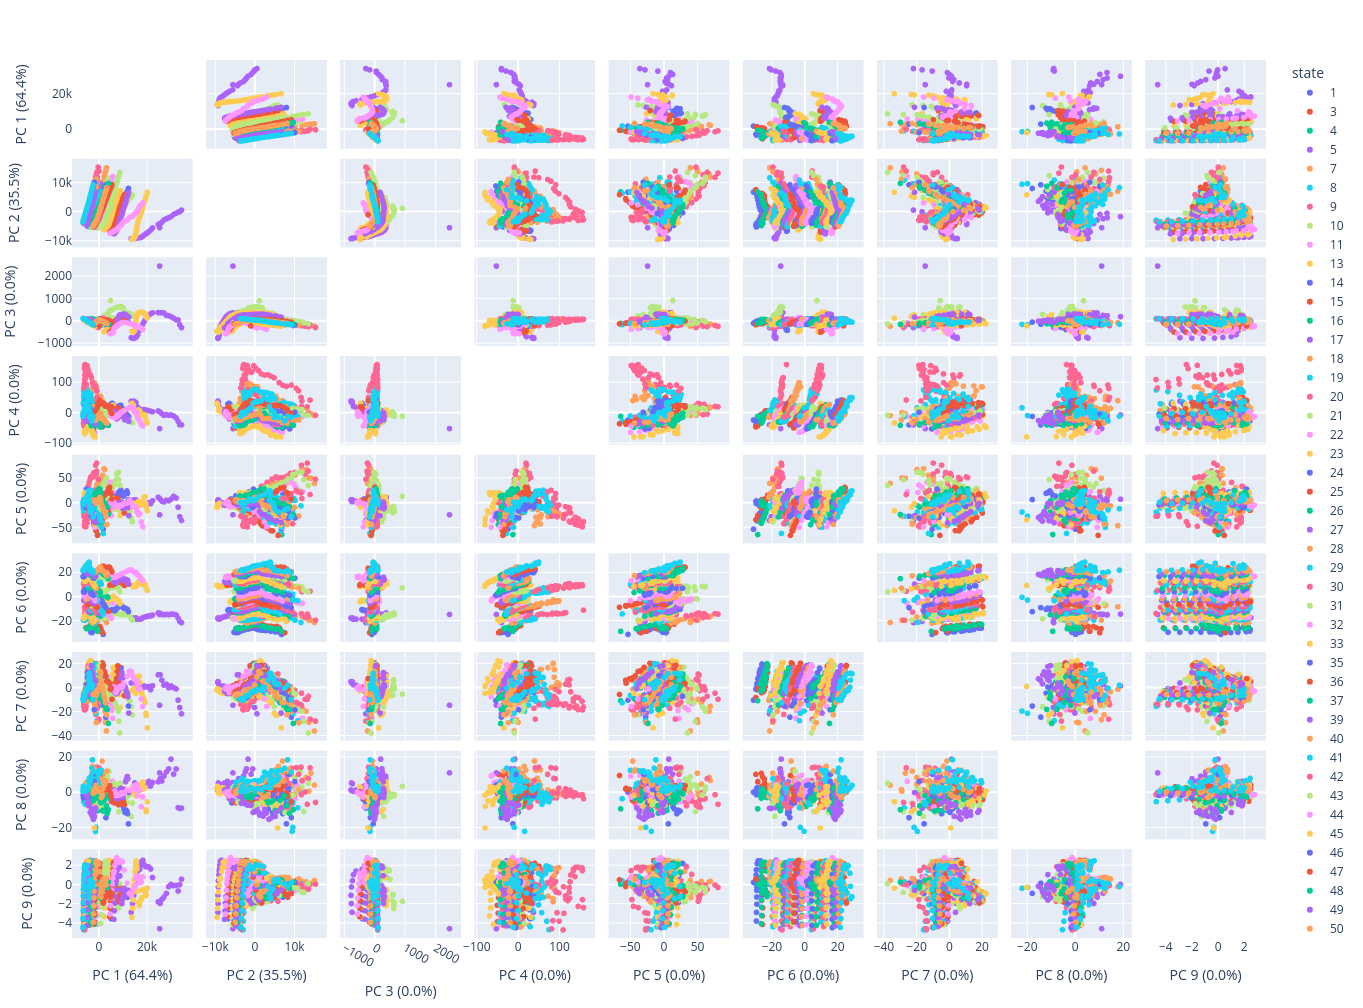
\includegraphics[width=.9\linewidth]{/home/buddhilw/EEL-USP/figs/PCA.png}}

🙏🙌 🤲 

\section{Fontes:}
\label{sec:org9c7932c}

\url{https://plotly.com/julia/pca-visualization/}
\url{https://r-data.pmagunia.com/dataset/r-dataset-package-plm-cigar}
\end{document}